%TWO BODY COLLISIONS
\newexp
\section*{Introduction}
Outside of Chicago at Fermilab, protons going $.999999\times c$ slam
into iron nuclei: a little collision problem involving conservation of momentum
and conservation of energy.
%     High energy physics often involves conservation of momentum and
%conservation of energy principles.  When high energy particles from an
%accelerator bombard the particles in a target we have a collision
%problem.  
The purpose of this experiment is to study the fundamentals of
collisions by analyzing the momentum and energy aspects of a two body
collision.  When the collision involves only two particles, the
trajectories of the particles before and after the collision lie in a
plane.  Therefore analysis in two dimensions is all that is necessary
to exactly solve this problem.% involving a two body collision.
\begin{figure}
\begin{center}
{\resizebox{3in}{!}{{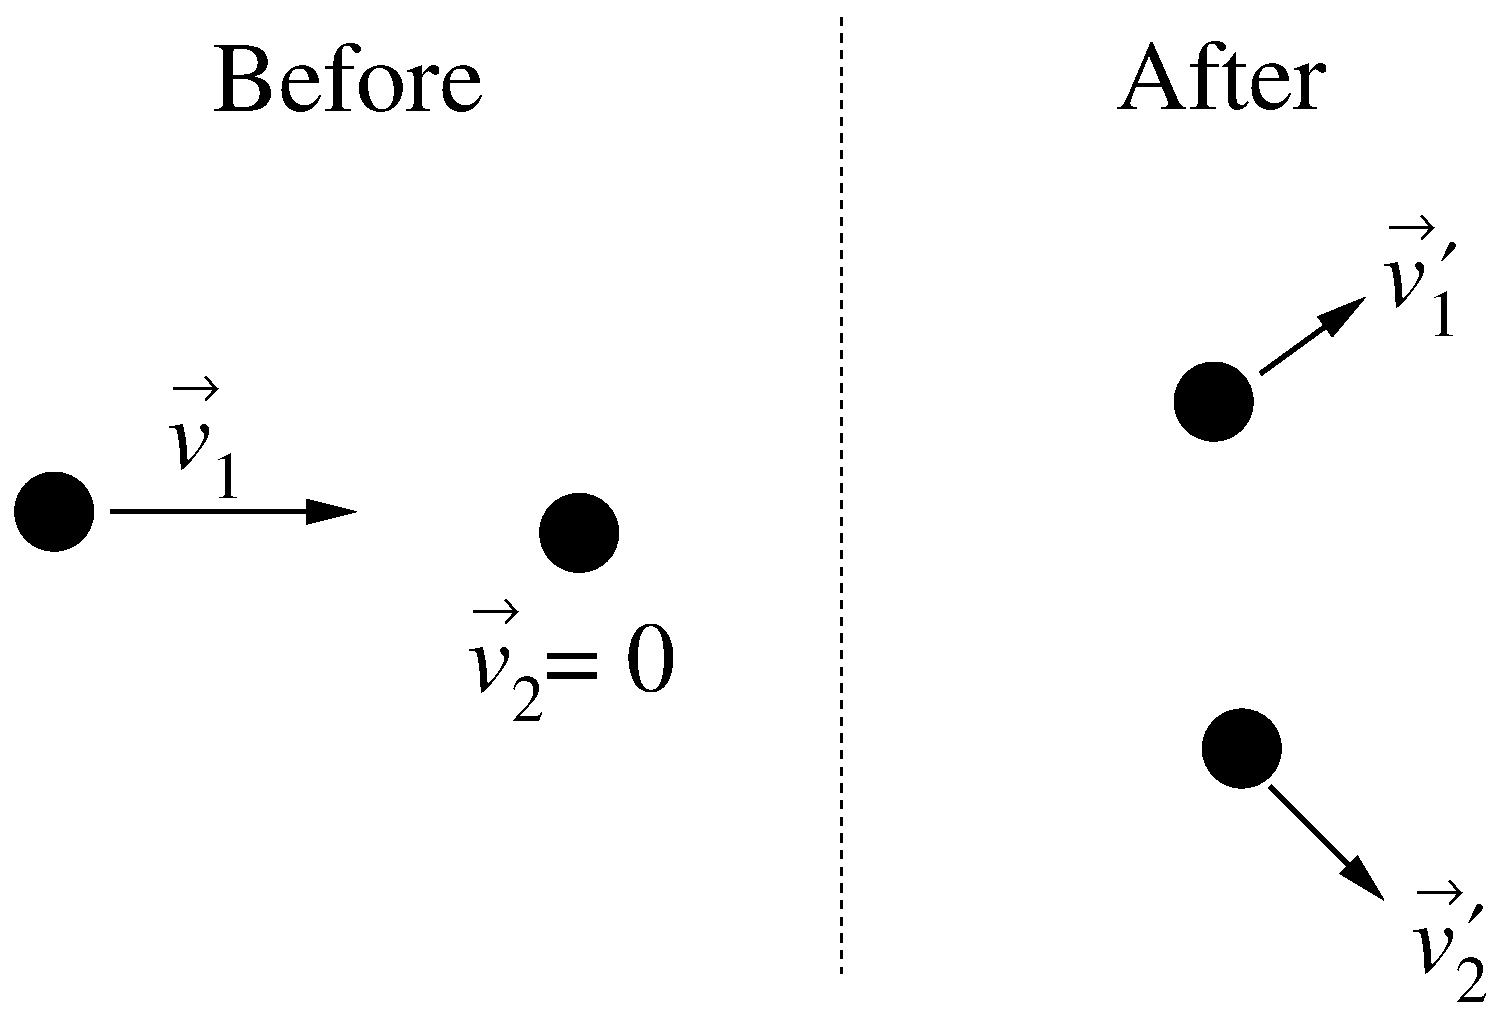
\includegraphics{2-body.defs.eps}}}}
\end{center}
%\vspace{2.5in}
%\special{ps:fig6_1.ps}
\caption{Diagram of a two body collision showing the situation before and
   after the collision.  \label{fig:tb1}}
\end{figure}

\section*{Analysis of Problem}
     In any collision, the total momentum of the colliding bodies is
unchanged by the collision.  Consider the case of a steel ball of mass
$m_{1}$ moving with velocity $\vec{\,v}_{1}$ colliding with mass $m_{2}$ initially at
rest.  (See Figure~\ref{fig:tb1}.)
After the collision the masses move off with velocities $\vec{\,v}_{1}'$ and $\vec{\,v}_{2}'$.
The law of conservation of momentum demands that the total momentum
before the collision, $\vec{P}$, is equal to the total momentum after the
collision, $\vec{P'}$.
\[
\vec{P} = \vec{P'}
\]
or
\begin{equation}
m_{1} \vec{\,v}_{1}  = m_1 \vec{\,v}_{1}' + m_2 \vec{\,v}_{2}'  \label{eq:tb1}
\end{equation}
     Remember that this vector equation actually represents
three equations, one for each coordinate direction.  In this experiment
we will observe collisions in two dimensions and only two of the three
equations will be used.  If the colliding objects are in the $x$-$y$ plane
we can write:
\begin{equation}
P_{x} = P_{x}' \qquad : \qquad m_1 v_{1x} = m_1 v_{1x}' + m_2 v_{2x}'
    \label{eq:tb2a}
\end{equation}
and
\begin{equation}
P_{y} = P_{y}' \qquad : \qquad m_1 v_{1y} = m_1 v_{1y}' + m_2 v_{2y}'
    \label{eq:tb2b}
\end{equation}
Here the $x$, $y$ subscripts denote the component of velocity along the $x$
 and $y$
axes.  It is convenient to set up the coordinate system so that $v_{1y} = 0$.
The Equations~\ref{eq:tb2a}~and~\ref{eq:tb2b} hold for any two dimensional
collision with one particle initially at rest.

     Kinetic energy is not necessarily conserved in a collision.  In the
case of two colliding steel balls about 10\% of the initial kinetic
energy is converted to heat and sound during the collision.  The total
kinetic energy before the collision in Figure~\ref{fig:tb1} is given by
\begin{equation}
E = {{1} \over {2}} \, m_1 v_{1}^{2}  \label{eq:tb3}
\end{equation}
 After the collision the total kinetic energy is
\begin{equation}
E' = {{1} \over {2}} \, m_1 \left( v_{1}' \right)^{2} + {{1} \over {2}} \,
      m_2 \left( v_{2}' \right)^{2}  \label{eq:tb4}
\end{equation}
 The percentage energy lost in the collision is
\begin{equation}
\mbox{\% loss} = {{E - E'} \over {E}} \times 100\%  \label{eq:tb5}
\end{equation}
     In this experiment we will use a curved aluminum ramp to accelerate
a steel ball and shoot it horizontally.  This ball strikes a second ball
at the end of the ramp.  Immediately after the collision both balls will
be traveling nearly horizontally; but they will quickly fall to the
floor because of the effect of gravity.  The time it takes to fall to
the floor is independent of the horizontal velocities or the masses of
the balls.  Therefore the horizontal displacement $d$ of either ball from
the point of collision is directly proportional to $v'$, the velocity of
that ball immediately after the collision.
\begin{equation}
v' = {d\over t}  \label{eq:tb6}
\end{equation}
where $t$ is the constant fall-time that 
is independent of the mass or horizontal velocity of the ball.
Calculations are much simplified if we invent a unit of time
(a {\em shake}) exactly equal to $t$.  Then $d$ is directly the
velocity in units of cm per shake.

%      In this experiment we will deal with relative measurements and
% simply forget about the constant $C$ even though it has units.  We will
% measure a quantity proportional to the velocities $v'$ of the balls by
% measuring the horizontal distance they travel after the collision.  In a
% sense we are measuring velocity in centimeters (per fall-time).  This procedure may seem
% a bit unusual, but remember we are simply ignoring the constant $C$ in
% Equation~\ref{eq:tb6} which is the same for both balls and has the proper
% dimensions to make the units come out correctly.

\section*{Experimental Procedure}
     Make sure that the apparatus is securely clamped to the lab table.
({\bf NOTE:}  Be sure to use the large bench clamps --- ordinary C clamps don't
seem to hold the apparatus securely enough.)  Tape a large piece of
paper to the floor near the lab table.  Choose two
steel balls of equal diameter (the 1/2 inch balls work well) and weigh
each ball to make sure that their masses do not differ by more than a
few percent.  This way you need not worry about which ball is which
during the experiment.

%    As a released ball rolls down the ramp, gravitional potential
%    energy is converted into kinetic energy.  If the center of mass
%    of the ball falls some vertical distance $\Delta z$, you might conclude
%    that the horizontal speed at the bottom of the ramp was given by:
%    \[
%    mg \: \Delta z = 0.5 m v^{2}
%    \]
%    In fact some of the gravitional potential energy rotational kinetic
%    energy, so as a result the horizontal velocity is reduced and is given by:
%    \[
%    mg \: \Delta z = 0.7 m v^{2}
%    \]
    
Mark a spot on the ramp and  release a ball from that spot.
and let it roll down the
ramp and strike the floor.  Release the ball smoothly without spinning or
pushing it. 
%Do not release the ball from the top
%of the ramp\ldots this gives poor results.  The height should be less than
%8 vertical cm from the table top. 
Now that you know where the ball will hit the floor, place a piece of
carbon paper (carbon side down) at that spot and release the
ball down the ramp again.    Repeat the procedure five times.
Estimate by eye the average
position of the marks made by the ball and the range of deviation.  
Record this distance and its deviation as
the initial velocity and its error.

{\bf NOTE:}  As the ball rolls down the ramp it acquires both translational
       and rotational kinetic energy.  As a result the translational
velocity is less than you might have calculated. The following equation, which you
       will learn to derive a bit later in the semester, takes into
       account both the translational kinetic energy of the center of
       mass, and the rotation of the spherical ball around an axis
       through the center of mass:
\[
mg \: \Delta z = 0.7 m v^{2}
\]
     Now we are ready to record the results of a two-body collision on
the same sheet of paper.  Place a target ball in one of the side dimples
at the bottom of the ramp.  Release the other ball from the same position on
the ramp that you used with the single ball trials.
Observe where each ball strikes the paper.  As before, place a
piece of carbon paper at these positions to record further collisions.
Lift the carbon paper and circle and number the pairs of marks after each
collision run.  Make five duplicate collision runs.

\section*{Analysis of the Data}
\begin{figure}
\begin{center}
{\resizebox{5in}{!}{{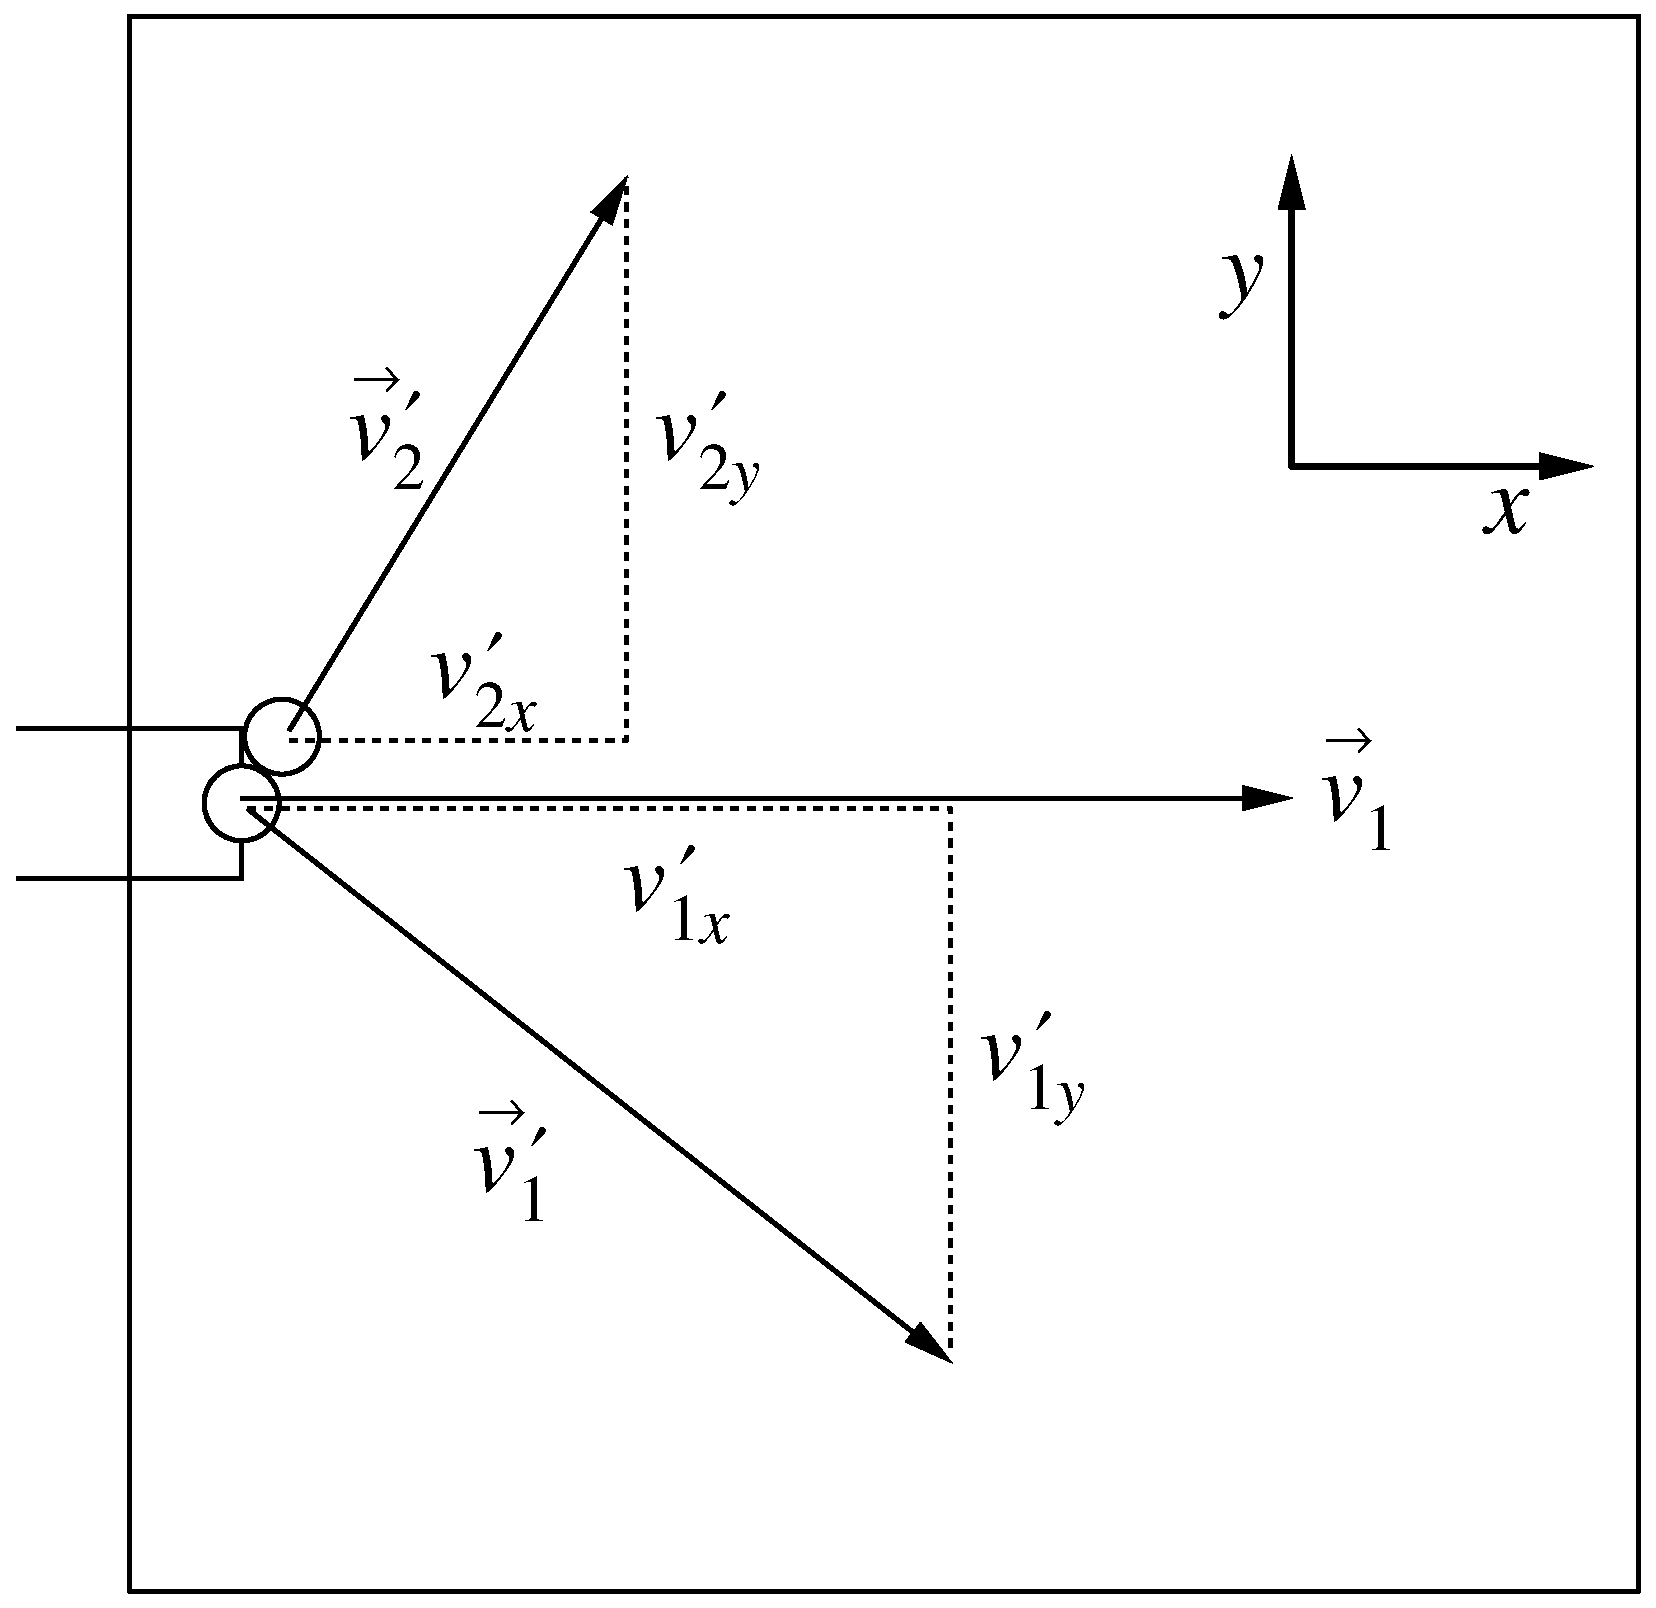
\includegraphics{2-body.coord.eps}}}}
\end{center}
%\vspace{3.375in}
%\special{ps:fig6_2.ps}
\caption{Coordinate system to be used in analyzing the data.  \label{fig:tb2}}
\end{figure}
     Using the coordinate system shown in Figure~\ref{fig:tb2} with the origin
directly below the collision point, measure the $x$ and $y$ components
of each of the ball's velocity after the collision in units of cm/shake.  From
this information, calculate the components of the momentum for each ball
and the total momentum after the collision.  Again we can simplify
our calculations by inventing a new unit of mass, a {\em steely}, exactly
equal to the mass of the steel balls.  The
momentum vector (in units of ${\rm steely\cdot cm/shake}$) is
numerically equal to the $x$ and $y$ components of the displacement.
The law of conservation of momentum now looks like a law of
conservation of the components of displacement.
Compare the $x$ and $y$ components of the total momentum
after the collision to the total momentum before the collision.  To what
accuracy do your measurements confirm that $P_{x}$ and $P_{y}$ are conserved
in the collision?

     Use your velocity data to calculate the initial and final kinetic
energy of each ball (in units of ${\rm steely\cdot cm^2/shake^2}$).  Calculate the total initial
and final kinetic energy of the balls.  What percentage of energy is
lost to heat and sound during the collision?  (Note that percentage energy lost
contains no funny units [or any units at all], and hence is exactly the same
as what you would have calculated if you'd gone through the bother of using normal
units.)

     It is possible to determine the mass of an object by observing the
effects of a collision of that object with an object of known mass and
velocity.  This is the method used by Chadwick to measure the mass of
the neutron in 1932.  Devise an experiment, based on conservation of
momentum principles to measure the mass of a marble. Remember to adjust
the holder height to make room for the larger marble.
To what accuracy does your experimental marble
mass agree with the measured mass of the marble?

\section*{Laboratory Report}
An acceptable laboratory report should include the following:
\begin{enumerate}
\item A brief description of your experimental procedure.
\item Sample computations.
\item Table listing the measured components of momentum.
\item A comparison of final and initial momentum, listed by components.
\item A calculation of percent kinetic energy lost.
\item Answers to all questions on the lab instruction
          sheet.
\item A description of your mass determination experiment.
\item Calculation and discussion of experimental error.
\end{enumerate}

\section*{Conclusions}
List all your numerical results and their uncertainties in a carefully
constructed table, and discuss them in detail.  For example, was momentum
conserved within the limits of experimental error?  Energy?
Comment on the amount of energy lost during the collision and on the
accuracy of your determination of the unknown mass.  Mention any sources of
error, both systematic and random.

\section*{Critique of Lab}
     Follow the suggestions given in the Introduction to the
Laboratory Manual.

